\lecture{16 \& 17}{2. -- 7. April 2025}{Phase diagrams, Pt: 2 \& 3}


\subsection{Development of microstructure in eutectic alloys}
Depending on the composition, several different types of microstructure are possible for the slow cooling of alloys belonging to binary eutectic systems.

The first case is for compositions ranging between a pure component and the maximum solid solubility for that component at room temperature. For e.g. a lead-tin system, this includes lead-rich alloys containing between 0 and about \qty{2}{wt}\% Sn (for the $\alpha$-phase solid solution) and also between approximately \qty{99}{wt}\% Sn and pure tin (for the $\beta$-phase). 

\begin{figure} [ht]
  \centering
  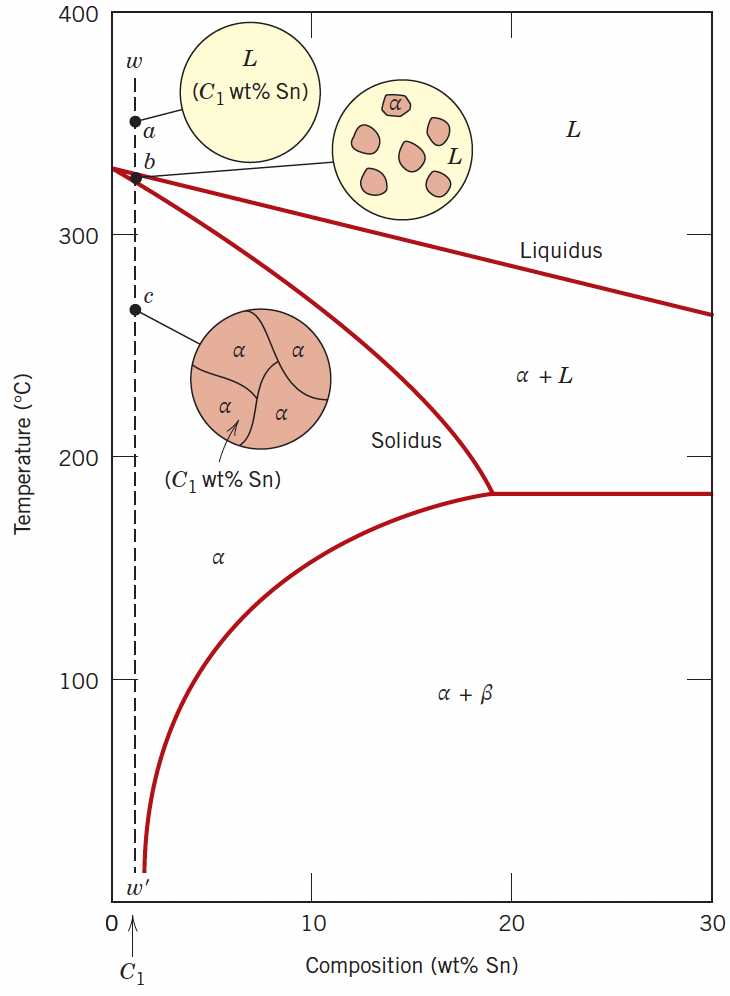
\includegraphics[width=0.35\linewidth]{./figures/f16_1.png}
  \caption{Phase diagram for lead-tin}
  \label{fig:f16_1}
\end{figure}
For example, consider an alloy of composition $C_1$ (\textbf{\autoref{fig:f16_1}}) as it is slowly cooled from a temperature within the liquid-phase region, say \qty{350}{\celsius}; this corresponds to moving down the dashed vertical line $ww'$ in the figure. The alloy will remain totally liquid and of composition $C_1$ until we cross the liquidus line at approximately \qty{330}{\celsius}, at which time the solid $\alpha$-phase begins to form. While passing through this narrow $\alpha + L$-phase region, solidification proceeds in the same manner as was described for the copper-nickel alloy in the previous section -- i.e., with continued cooling, more of the solid $\alpha$ forms. Furthermore, liquid- and solid-phase compositions are different, which follow along the liquidus line and solidus phase boundaries, respectively. Solidification reaches completion with a uniform composition of $C_1$, and no subsequent changes occur upon cooling to room temperature. This is the point $c$ on \textbf{\autoref{fig:f16_1}}.

\begin{figure} [ht]
  \centering
  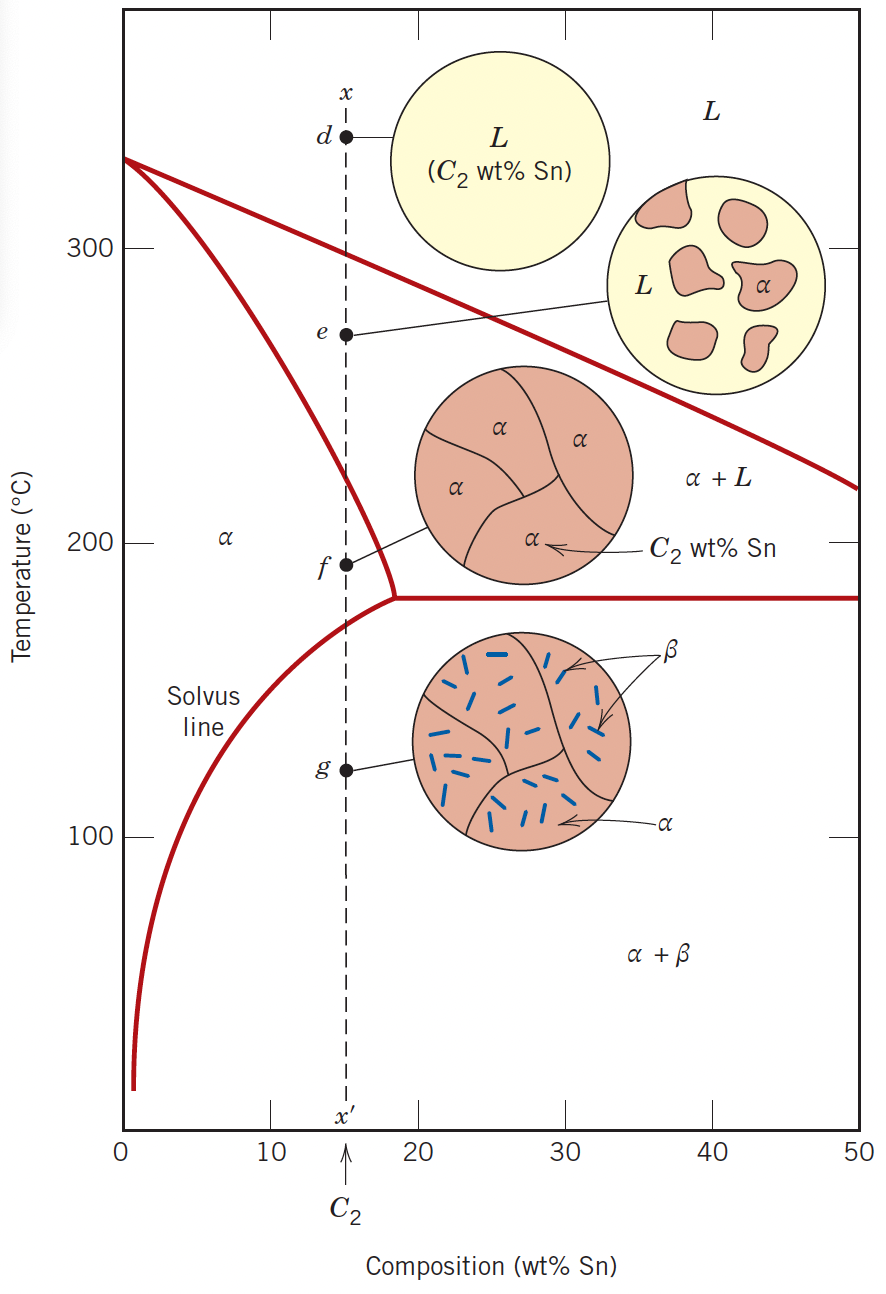
\includegraphics[width=0.35\linewidth]{./figures/f16_2.png}
  \caption{Phase diagram for lead-tin with a new composition}
  \label{fig:f16_2}
\end{figure}
The second case considered is for compositions that range between the room temperature solubility limit and the maximum solid solubility at the eutectic temperature. For the lead-tin system, these compositions extend from about 2 to \qty{18,3}{wt}\% Sn (for lead-rich alloys) and from \num{97,8} to approximately \qty{99}{wt}\% Sn (for tin-rich alloys). We will now examine an alloy of composition $C_2$ (\textbf{\autoref{fig:f16_2}}) as it is cooled along the vertical line $x x'$. Down to the intersection of $ x x'$ and the solvus line, changes that occur are similar to the previous case as we pass through the corresponding phase regions (as demonstrated by the points $d, e,$ and $f$). Just above the solvus intersection, at point $f$, the microstructure consists of $\alpha$ grains of composition $C_2$. Upon crossing the solvus line, the $\alpha$ solid solubility is exceeded, which results in the formation of small $\beta$-phase particles; these are indicated in the microstructure inset at point $g$. With continued cooling, these particles grow in size because the mass fraction of the $\beta$ phase increases slightly with decreasing temperature.

\begin{figure} [ht]
  \centering
  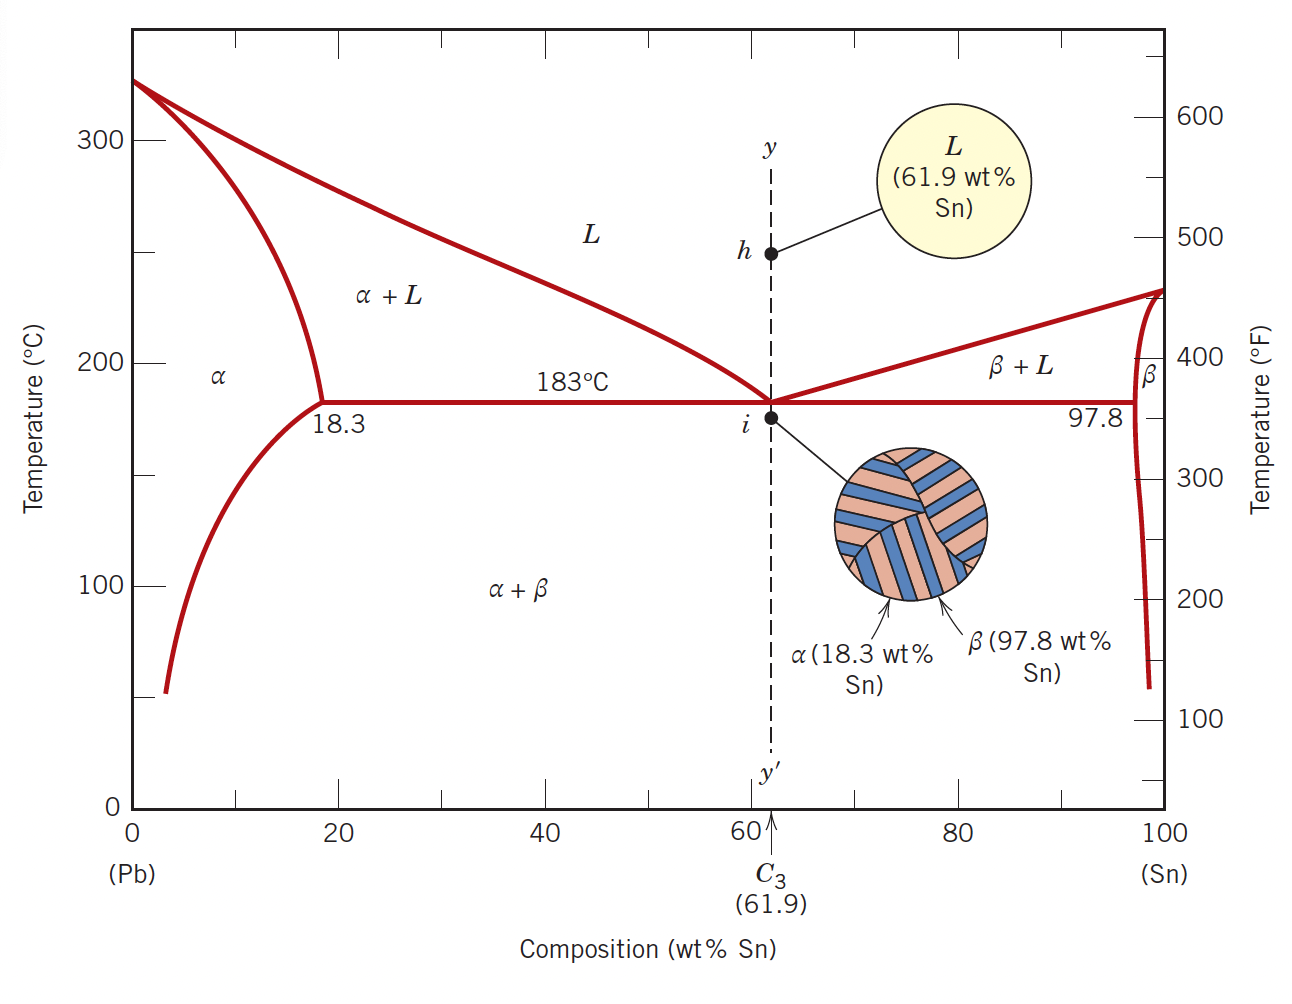
\includegraphics[width=0.5\linewidth]{./figures/f16_3.png}
  \caption{Phase diagram for lead-tin with a new composition once again}
  \label{fig:f16_3}
\end{figure}
The third case involves solidification of the eutectuc composition, \qty{61,9}{wt}\% Sn ($C_3$ in \textbf{\autoref{fig:f16_3}}). We consider an alloy having this composition that is cooled from a temperature within the liquid-phase region (e.g. \qty{250}{\celsius}) down the vertical line $yy'$. As the temperature is lowered, no changes occur until we reach the eutectic temperature, \qty{183}{\celsius}. Upon crossing the eutectic isotherm, the liquid transforms into the two $\alpha$ and $\beta$ phases. This transformation can be represented by the reaction:
\[ 
L(\qty{61,9}{wt}\% \text{ Sn}) \leftrightharpoons \alpha(\qty{18,3}{wt}\% \text{ Sn}) + \beta(\qty{97,8}{wt}\% \text{ Sn})
\]
in which the $\alpha$- and $\beta$-phase compositions are dictated by the eutectic isotherm end points. During this transformation, there must be a redistribution of the lead and tin components because the $\alpha$ and $\beta$ phases have different compositions, neither of which is the same as that of the liquid (as indicated in the above equation). This redistribution is accomplished by atomic diffusion. The microstructure of the solid that results from this transformation consists of alternating layers (sometimes called \textit{lammellae}) of the $\alpha$ and $\beta$ phases that form simultaneously during this transformation. This microstructure, represented schematically in \textbf{\autoref{fig:f16_3}} at point $i$, is called a \textit{eutectic structure} and is characteristic of this reacion. A subsequent cooling of the alloy from just below the eutectic to room temperature will only result in minor mictrostructural alterations.

\begin{figure} [ht]
  \centering
  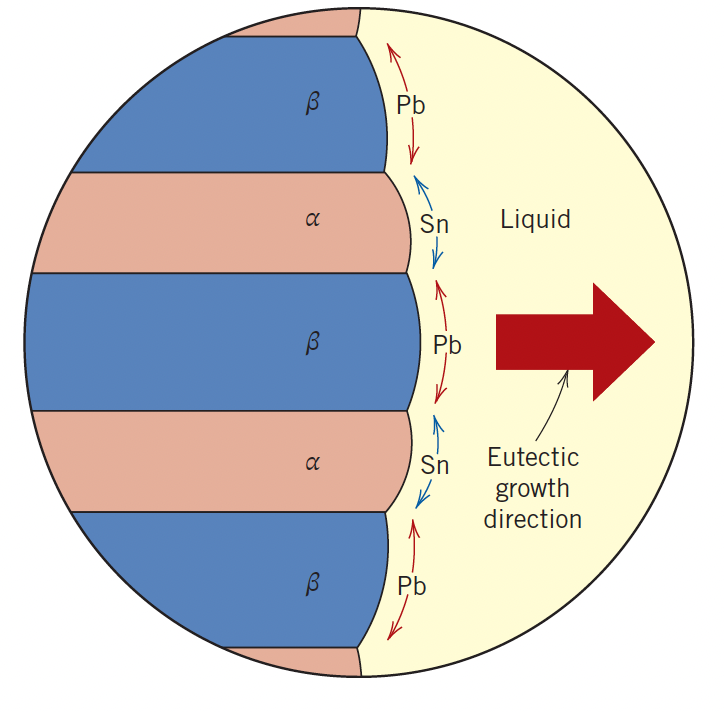
\includegraphics[width=0.35\linewidth]{./figures/f16_4.png}
  \caption{The formation of the eutectic structure for the lead-tin system}
  \label{fig:f16_4}
\end{figure}
The microstructural change that accompanies this eutectic transformation is represented schematically in \textbf{\autoref{fig:f16_4}}, which shows the $\alpha-\beta$ layeres eutectic growing into and replacing the liquid phase. This process of the redistribution of lead and tin occurs by diffusion in the liquid just ahead of the eutectic-liquid interface. The arrow indicated the directions of diffusion of lead and tin atoms; lead atoms diffuse towards the $\alpha$-phase layers because this $\alpha$ phase is lead-rich (\qty{18,3}{wt}\% Sn and \qty{81,7}{wt}\% Pb); conversely, the direction of diffusion of tin will be opposite. The eutectic structure forms in these alternating layers because, for this lamellar configuration, atomic diffusion of lead and tin need only occur over relatively short distances.

\begin{figure} [ht]
  \centering
  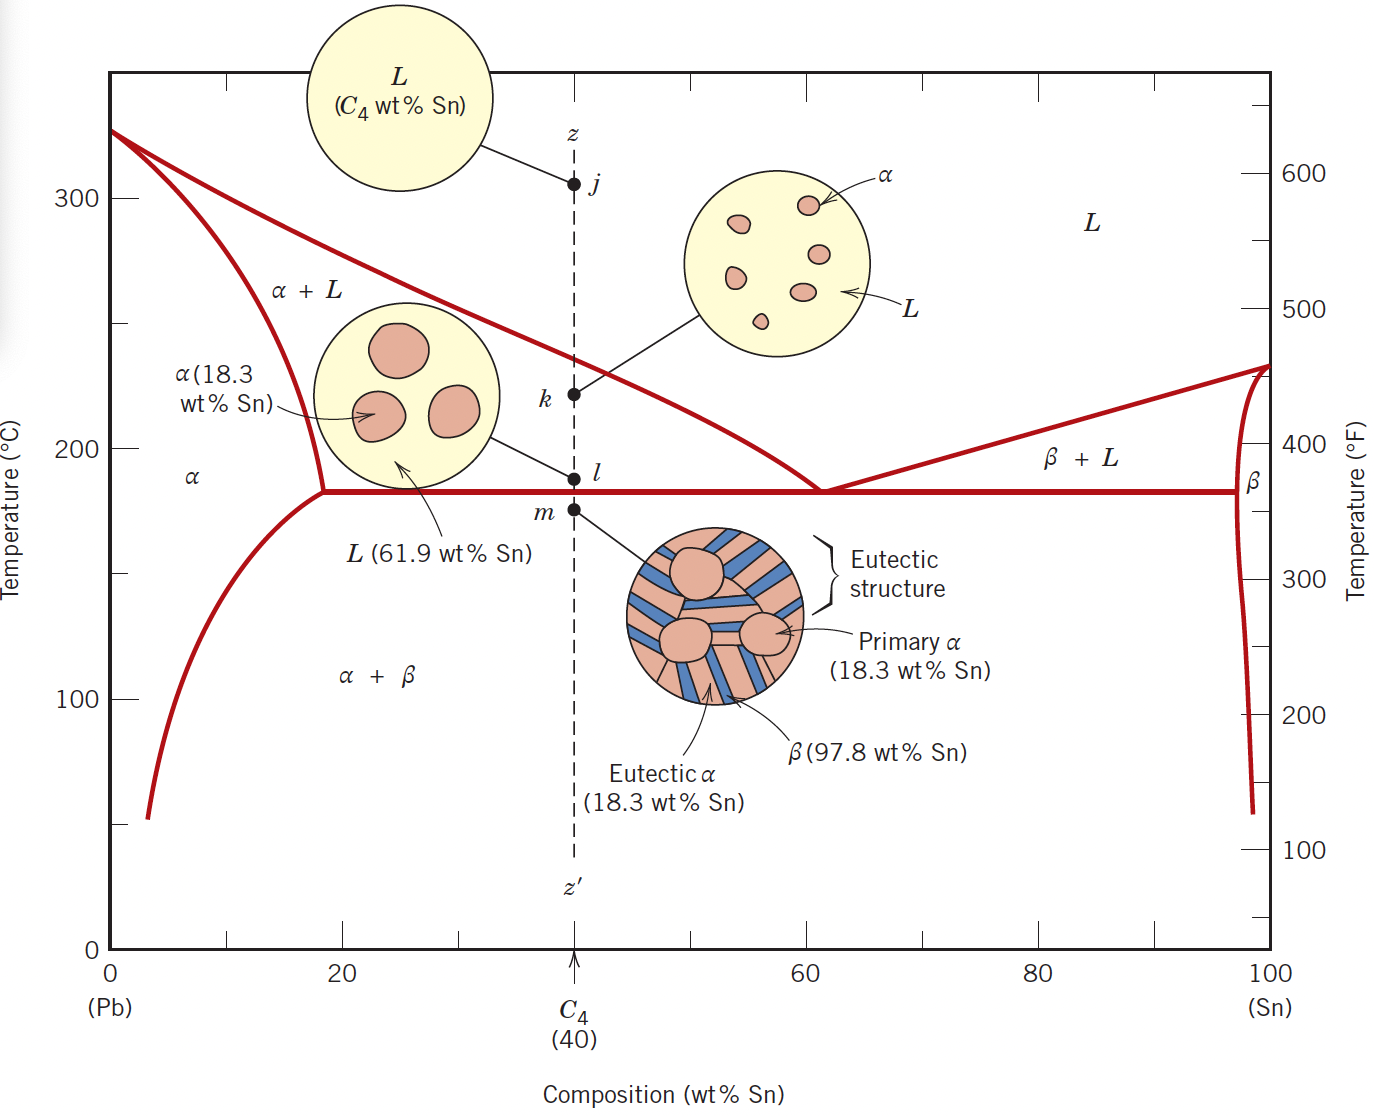
\includegraphics[width=0.45\linewidth]{./figures/f16_5.png}
  \caption{Phase diagram for the lead-tin system at yet another composition}
  \label{fig:f16_5}
\end{figure}
The fourth and final microstructural case for this system includes all compositions other than the eutectic that, when cooled, cross the eutectic isotherm. Consider, for example the composition $C_4$ (\textbf{\autoref{fig:f16_5}}), which lies to the left of the eutectic; as the temperature is lowered, we move down the line $zz'$, beginning at point $j$. The microstructural development between points $j$ and $l$ is similar to that for the second case, such that just prior to crossing the eutectic isotherm (point $l$), the $\alpha$ and liquid phases are present with compositions of approximately \num{18,3} and \qty{61,9}{wt}\% Sn, respectively, as determined from the appropriate tie line. As the temperature is lowered to just below the eutectic, the liquid phase, which is of the eutectic composition, transforms into the eutectic structure (i.e. alternating $\alpha$ and $\beta$ lamellae); insignificant changes occur with the $\alpha$ phase that is formed during cooling through the $\alpha + L$ region. This microstructure is also schematically shown at the inset point $m$ on \textbf{\autoref{fig:f16_5}}. This, the $\alpha$ phase is present both in the eutectic structure and also as the phase that formed while cooling through the $\alpha + L$ phase field. To distinguish one $\alpha$ from the other, that which resides in the eutectic structure is called \textit{eutectic} $\alpha$, whereas the other that formed prior to crossing the eutectic isotherm is termed \textit{primary} $\alpha$. 

When dealing with microstructures, it is sometimes convenient to use the term \textit{microconstituent} -- i.e., an element of the microstructure having an identifiable and characteristic structure. For example at point $m$ on \textbf{\autoref{fig:f16_5}}, there are two microconstituents -- primary $\alpha$ and the eutectic structure. Thus, the eutectic structure is a microconstituent even though it is a mixture of two phases because it has a distinct lamellar structure with a fixed ratio of the two phases.

\begin{figure} [ht]
  \centering
  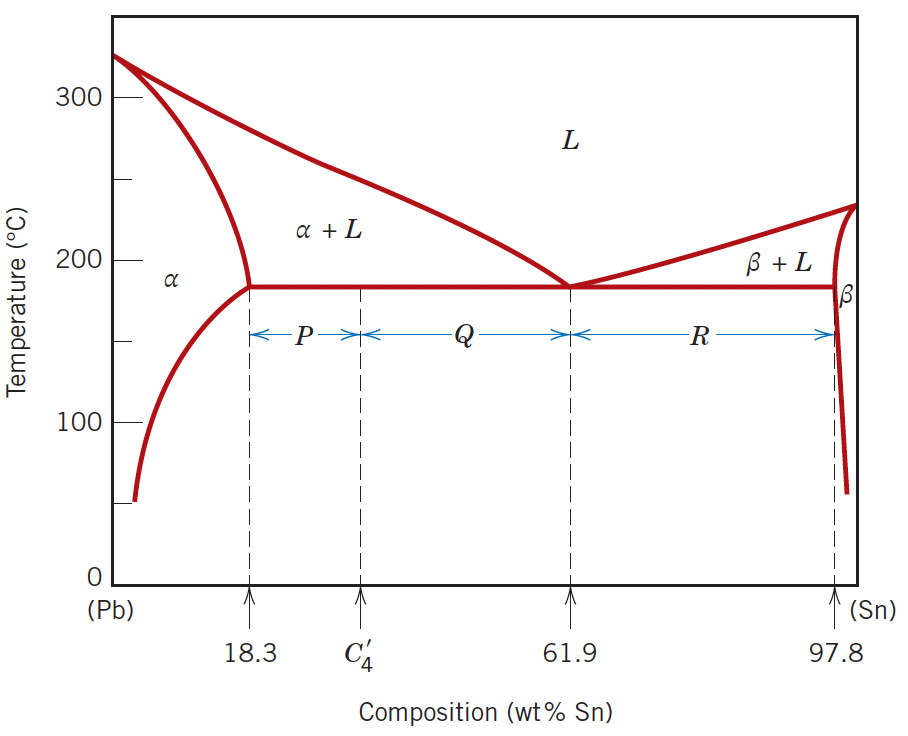
\includegraphics[width=0.5\linewidth]{./figures/f16_6.png}
  \caption{The lead-tin phase diaggram in whole}
  \label{fig:f16_6}
\end{figure}
It is indeed possible to compute the relative amounts of both eutectic and primary $\alpha$ microconstituents. Because the eutectic microconstituents always forms from the liquid having the eutectic composition, this microconstituent may be assumed to have a composition of \qty{61,9}{wt}\% Sn. Hence, the lever rule is applied using a tie-line between the $\alpha-\left(\alpha + \beta  \right)$ phase boundary (\qty{18,3}{wt}\% Sn) and the eutectic composition. For example, consider the alloy of composition $C_4'$ in \textbf{\autoref{fig:f16_6}}. The fraction of the eutectic microconstituent $W_e$ is just the same as the fraction of the liquid $W_L$ from which it transforms, or
\[ 
  W_e = W_L = \frac{P}{P+Q} = \frac{C_4' - \num{18,3}}{\num{61,9} - \num{18,3}} = \frac{C_4' - \num{18,3} }{\num{43,6}}
.\]
Furthermore, the fraction of primary $\alpha$, $W_{\alpha'}$, is just the fraction of the $\alpha$ phase that existed prior to the eutectic transformation or, from \textbf{\autoref{fig:f16_6}}:
\[ 
W_{\alpha'} = \frac{Q}{P+Q} = \frac{\num{61,9} - C_4'}{\num{61,9} - \num{18,3} } = \frac{\num{61,9} - C_4'}{\num{43,6} }
.\]
The fractions of \textit{total} $\alpha$ $W_{\alpha}$ (both eutectic and primary), and also of total $\beta$, $W_{\beta}$, are determined by use of the lever rule and a tie line the extends \textit{entirely across the $\alpha + \beta$ phase field}. Again, for an alloy having composition $C_4'$:
\begin{align*}
  W_{\alpha} &= \frac{Q + R}{P + Q + R} = \frac{\num{97,8} - C_{4}'}{\num{97,8} - \num{18,3}} = \frac{\num{97,8} - C_4'}{\num{79,5}} \\
  W_{\beta} &= \frac{P}{P + Q + R} = \frac{C_4' - \num{18,3} }{\num{97,8} - \num{18,3}} = \frac{C_4' - \num{18,3} }{\num{79.5} }
.\end{align*}
Analogous transformations and microstructures result for alloys having compositions to the right of the eutectic (i.e., between \num{61,9} and \qty{97,8}{wt}\% Sn). However, below the eutectic temperature, the microstructure will consist of the eutectic and primary $\beta$ microconstituents because, upon cooling from the liquid, we pass through the $\beta+ \text{liquid}$ phase field. 

When, for the fourth case represented in \textbf{\autoref{fig:f16_5}}, conditions of equilibrium are not maintained passing through the $\alpha$ (or $\beta$) + liquid phase region, the following consequences will be realized for the microstructure upon crossing the eutectic isotherm:
\begin{itemize}
  \item Grains of the primary microconstituent will be cored, that is, have a nonuniform distribution of solute across the grains
  \item The fraction of the eutectic microconstituent formed will be greater than for the equilibrium situation
\end{itemize}


\subsection{Equilibrium diagrams having intermediate phases or compounds}
The isomorphous and eutectic phase diagrams discussed thus far are relatively somple, but for many binary systems much more complex interactions arise. The eutectic systems discussed thus far only have two solid phases, $\alpha$ and $\beta$; these are sometimes termed \textit{terminal solid solutions} because they exist over composition ranges near the concentration extremes of the phase diagram. For other alloy systems, \textit{intermediate solid solutions} (or \textit{intermediate phases}) may be found at other than the two composition extremes. Such is the case for the copper-zinc system. Its phase diagram (\textbf{\autoref{fig:f16_7}}) may at first appear formidable because there are some invariant reactions similar to the eutectic that have not yet been discussed. In addition, there are six different solid solutions -- two terminal ($\alpha$ and $\eta$) and \textit{four} intermediate ($\beta, \gamma, \delta$, and $\epsilon$). The $\beta'$ phase is termed an \textit{ordered solid solution}, one in which the copper and zinc atoms are situated in a specific and ordered arrangement within each unit cell. The dashed boundaries near the bottom are dashed, as they have not been exactly determined yet. This is due to the fact that at low temperatures, diffusion rates are very slow, and inordinarily long times are required to attain equilibrium.

\begin{figure} [ht]
  \centering
  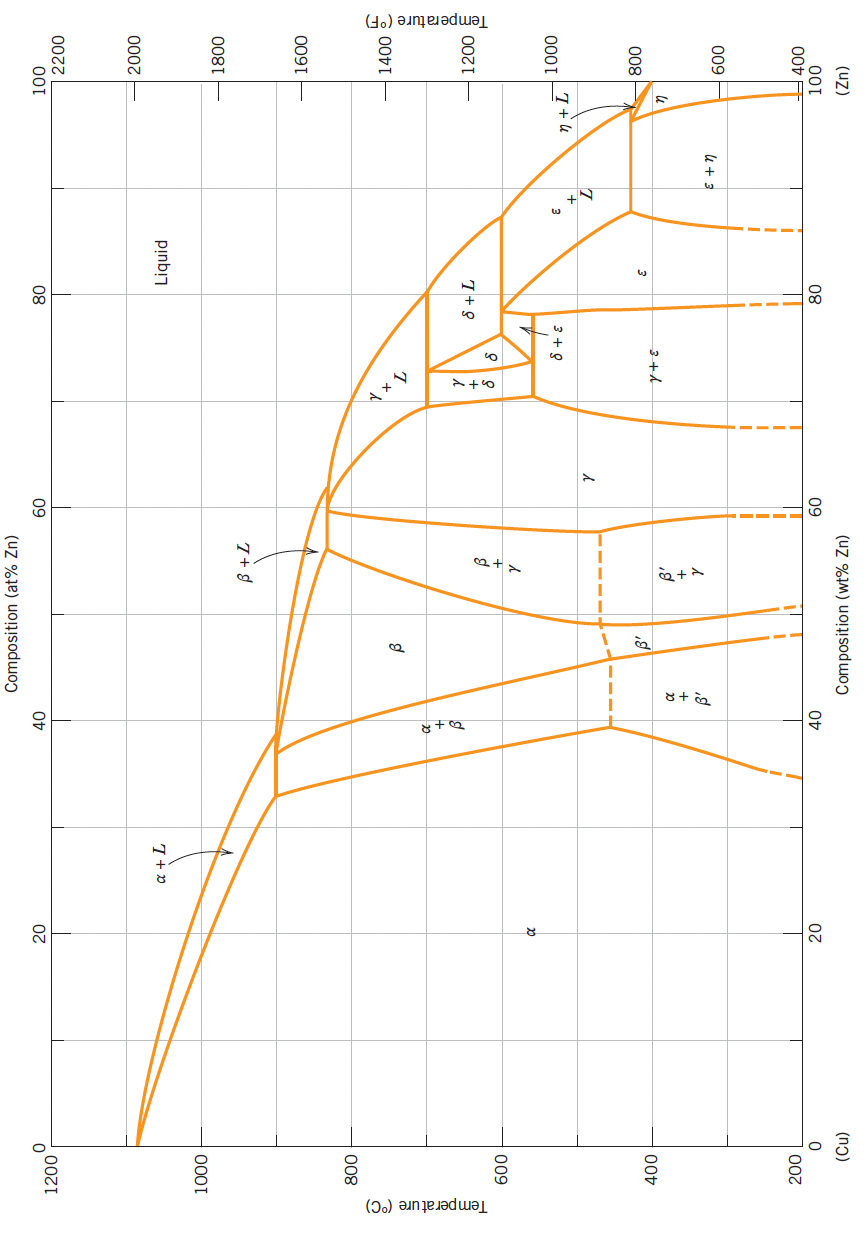
\includegraphics[width=0.35\linewidth]{./figures/f16_7.png}
  \caption{The copper-zinc phase diagram}
  \label{fig:f16_7}
\end{figure}

Commercial brass is a copper-rich copper-zinc alloy. E.g., Cartridge brass has a composition of \qty{70}{wt}\% Cu and \qty{30}{wt}\% Zn and therefore a microstructure consisting of a single $\alpha$ phase.

For some systems, discrete intermediate compounds rather than solid solutions may be found on the phase diagram, and these compounds have distinct chemical formulas; for metal-metal systems, they are called \textit{intermetallic compounds}. E.g., consider the magnesium-lead system (\textbf{\autoref{fig:f16_8}}). The compound $\mathrm{Mg}_2 \mathrm{Pb}$ has a composition of \qty{19}{wt}\% Mg and \qty{81}{wt}\% Pb and is represented as a vertical line on the diagram, rather than as a phase region of finite width; hence, $\mathrm{Mg}_2 \mathrm{Pb}$ can exist by itself only at this precise composition.

\begin{figure} [ht]
  \centering
  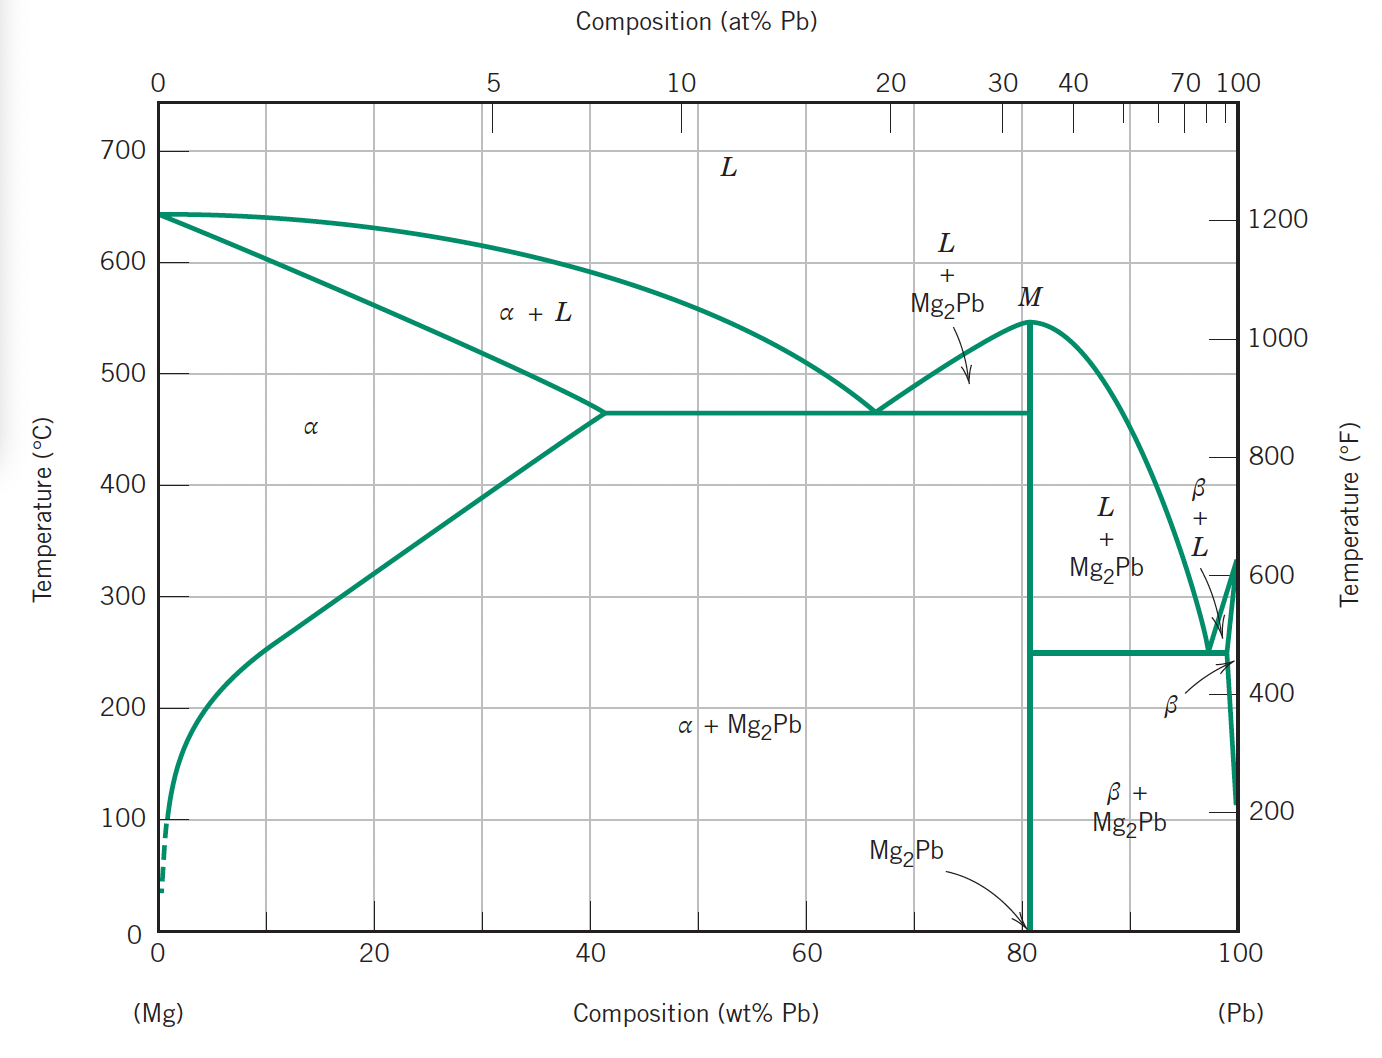
\includegraphics[width=0.35\linewidth]{./figures/f16_8.png}
  \caption{The magnesium-lead phase diagram}
  \label{fig:f16_8}
\end{figure}

Several other characteristics are worth noting for this magnesium-lead system. First, the compound $\mathrm{Mg}_2 \mathrm{Pb}$ melts at approximately \qty{550}{\celsius}, as indicated by point $M$ on \textbf{\autoref{fig:f16_8}}. Also, the solubility of lead in magnesium is rather extensive. However, the solubility of magneisum in lead is extremely limited. Finally, this phase diagram may be thought of as two simple eutectic diagrams joined back to back, one for the Mg-$\mathrm{Mg}_2 \mathrm{Pb}$ system and the other for $\mathrm{Mg}_2 \mathrm{Pb}$-Pb; as such, the compound $\mathrm{Mg}_2 \mathrm{Pb}$ is really considered to be a component.


\subsection{Eutectoid and peritectic reactions}
In addition to the eutectic, other invariant reactions involving three different phases are found for some alloy systems. One of these occurs for the copper-zinc system (\textbf{\autoref{fig:f16_7}}) at \qty{560}{\celsius} and \qty{74}{wt}\% Zn and \qty{26}{wt}\% Cu. A portion of the phase diagram in this vicinity is enlarged in \textbf{\autoref{fig:f16_9}}. Upon cooling, a single solid $\delta$ phase transforms into two other solid phases $\gamma$ and $\epsilon$ and v.v. for heating according to the reaction:
\[ 
\delta \leftrightharpoons \gamma + \epsilon
.\]
This is called a \textit{eutectoid reaction}; the eutectoid point is labelled $E$ on \textbf{\autoref{fig:f16_9}}, The feature dustinguishing eutectoid from eutectic is that one solid phase instead of a liquid transforms into two other solid phases at a single temperature. 

\begin{figure} [ht]
  \centering
  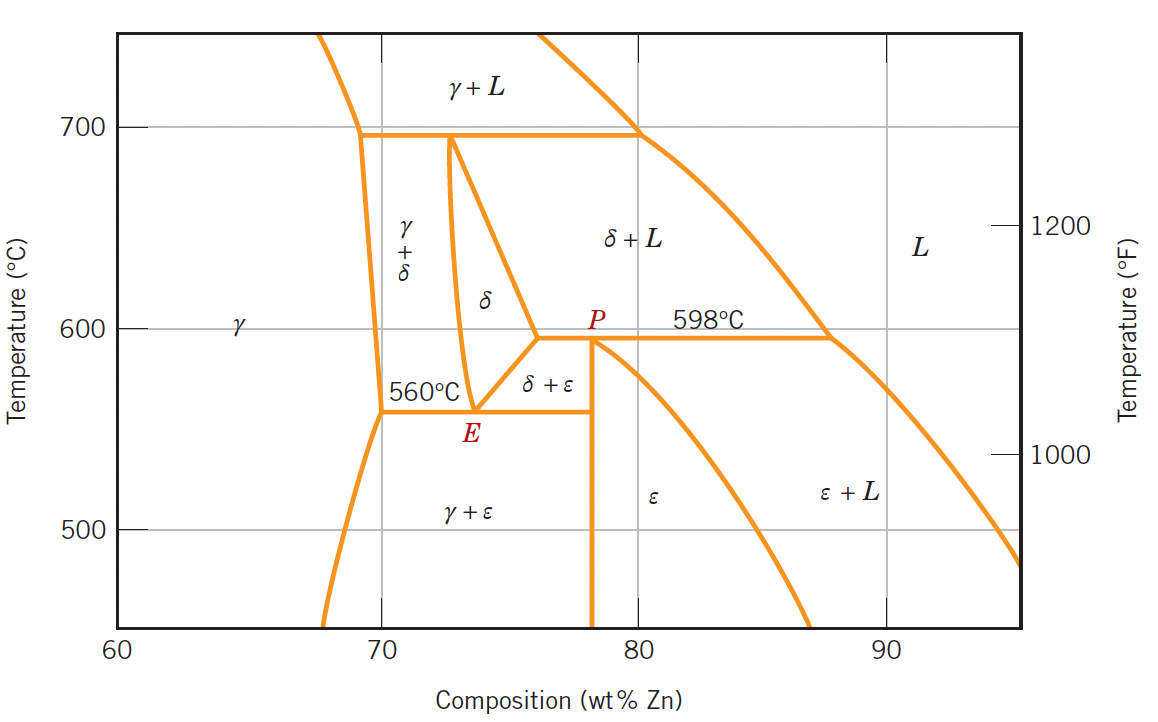
\includegraphics[width=0.5\linewidth]{./figures/f16_9.png}
  \caption{The copper-zinc diagram zoomed in near the peritectic and eutectoid region}
  \label{fig:f16_9}
\end{figure}

A \textit{peritectic reaction} is another invariant reaction involving three phases at equilibrium. With this reaction, upon heating, one solid phase transforms into a liquid phase and another solid phase. A peritectic exists for the copper-zinc system at point $P$ on \textbf{\autoref{fig:f16_9}}. This reaction is as follows:
\[ 
\delta + L \leftrightharpoons \epsilon
.\]
The low-temperature solid phase may be an intermediate solid solution (e.g., $\epsilon$ in the preceding reaction), or it may be a terminal solid solution. One of the latter peritectics exists at about \qty{97}{wt}\% Zn at \qty{435}{\celsius} (see \textbf{\autoref{fig:f16_7}}), where the $\eta$ phase, when heated, transforms into $\epsilon$ and liquid phases. Three other peritectics are found for the Cu-Zn system, the reactions of which involve $\beta, \delta,$ and $\gamma$ intermediate solid solutions as the low-temperature phases that transform upon heating. 


\subsection{Congruent phase transformations}
Phase transformations may be classified according to whether there is any change in composition for the phases involved. Those for which there are no compositional changes are said to be \textit{congruent transformations}, e.g. melting of pure metals. Conversely, for \textit{incongruent transformations}, at least one of the phases experiences a change in composition, e.g. melting of an alloy or eutectic/eutectoid reactions.

\begin{figure} [ht]
  \centering
  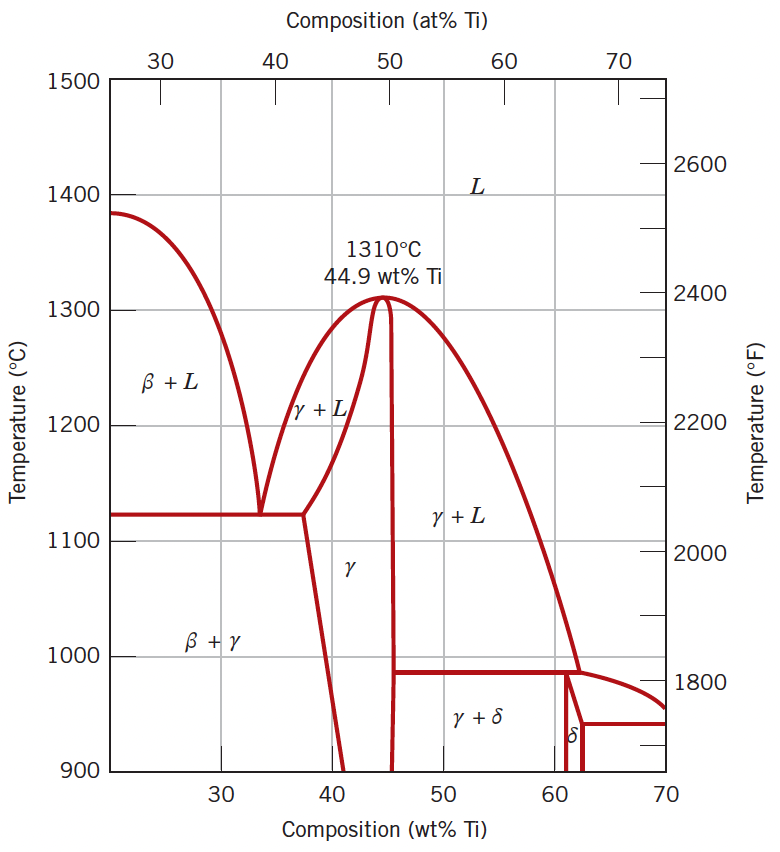
\includegraphics[width=0.5\linewidth]{./figures/f16_10.png}
  \caption{Portion of the phase diagram for nickel-titanium}
  \label{fig:f16_10}
\end{figure}

Intermediate phases are sometimes classified on the basis of whether they melt congruently or incongruently. The intermetallic compound $\mathrm{Mg}_2 \mathrm{Pb}$ melts congruently at the point designated $M$ on \textbf{\autoref{fig:f16_8}}. For the nickel-titanium system on \textbf{\autoref{fig:f16_10}}, there is a congruent melting point for the $\gamma$ solid solution that corresponds to the point of tangency for the pairs of liquidus and solidus lines at \qty{1310}{\celsius} and \qty{44,9}{wt}\% Ti. The peritectic reaction is an example of incengruent melting for an intermediate phase. 

\subsection{The Gibbs phase rule}
One of the most important laws of thermodynamics when talking about phase diagrams is the \textit{Gibbs phase rule}. This rule represents a criterion for the number of phases that coexist within a system at equilibrium and is expressed by the simple equation:
\[ 
P + F = C + N
\]
Where $P$ is the number of phases present. $F$ is the number of \textit{degrees of freedom} or the number of externally controlled variables (e.g., temperature, pressure, composition) that must be specified to define the state of the system completely. I.e., $F$ is the number of these variables that can be changed independently without altering the number of phases that coexist at equilibrium. The parameter $C$ represents the number of components in the system. Components are normally elements or stable compounds and, in the case of phase diagrams, are the materials at the two extremes of the composition axis. Finally $N$ is the number of noncompositional variables (e.g., temperature and pressure)

This rule will now be demonstrated by applying it to binary temperature-composition phase diagrams. More specifically the copper-silver system previously discussed. Because pressure is constant (\qty{1}{atm}), the parameter $N$ is 1, as temperature is the only noncompositional \textit{variable}. Therefore we have:
\[ 
P + F = C + 1
.\]
The number of components $C$ is 2 (Cu and Ag):
\[ 
P + F = 2+1 = 3
\]
or:
\[ 
F = 3-P
.\]
Let us consider the case of single-phase fields on the phase diagram (e.g., $\alpha, \beta$, and liquid regions). Because only one phase is present $P = 1$ and
\[ 
F = 3-P = 3-1 = 2
.\]
Therefore we must specify two parameters to completely describe the characteristics of any alloys that exists within one of these phase fields. These two parameters are composition and temperature, which locate, respectively, the horizontal and vertical positions of the alloy respectively. 

For the situation in which two phases coexist -- e.g., $\alpha + L, \beta + L,$ and $\alpha + \beta$ phase regions -- the phase rule stipulates that we have one degree of freedom because:
\[ 
F = 3 - P = 3- 2 = 1
.\]
Thus, it is necessary to specify either temperature or the composition of one of the phases to completely define the system. 

For binary systems, when three phases are present, there are no degrees of freedom because:
\[ 
F = 3 - P = 3 - 3 = 0
.\]
This means that the composition of all three phases -- as well as the temperature -- are fixed. This condition is met for a eutectic isotherm.


\subsection{The iron-iron carbide phase diagram}
A portion of the iron-iron carbide phase diagram is shown on \textbf{\autoref{fig:f16_11}}. Pure iron, upon heating, experiences two changes in crystal structure before it melts. At room temperature, the stable form, called \textit{ferrite}, or $\alpha$-iron, has a BCC crystal structure. Ferrite experiences a polymorphic transformation to FCC \textit{austenite}, or $\gamma$-iron ar \qty{912}{\celsius}. This austenite persists to \qty{1394}{\celsius} at which temperature the FCC austenite reverts back to a BCC phase known as $\delta$-ferrite, which finally melts at \qty{1538}{\celsius}. All these changes are apparent along the left vertical axis of \textbf{\autoref{fig:f16_11}}

\begin{figure} [ht]
  \centering
  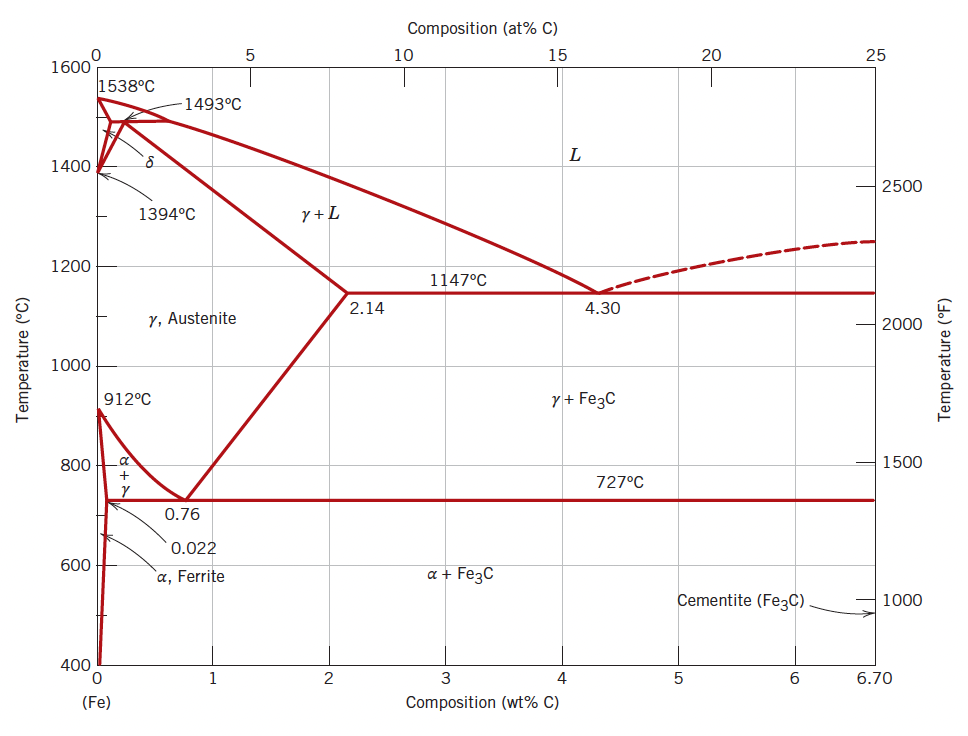
\includegraphics[width=0.5\linewidth]{./figures/f16_11.png}
  \caption{Portion of the iron-iron carbide phase diagram}
  \label{fig:f16_11}
\end{figure}

The composition axis on \textbf{\autoref{fig:f16_11}} extends only to \qty{6,70}{wt}\% C; at this concentration the intermediate compound iron carbide, or \textit{cementite} ($\mathrm{Fe}_3 \mathrm{C}$) is formed, which is represented by a vertical line on the phase diagram. Thus, the iron-carbon system may be divided into two parts: an iron rich portion (\textbf{\autoref{fig:f16_11}}) and the other for composition from \qty{6,70}{wt}\% C and up (not shown).

Carbon is an interstital impurity in iron and forms a solid solution with each of $\alpha$-, $\gamma$- and $\delta$-ferrites. In the BCC $\alpha$-ferrite, only small concentrations of carbon are soluble (max is around \qty{0,022}{wt}\% C at \qty{727}{\celsius}). The limited solubility is explained by the shape and size of the BCC interstitial positions, which make it difficult to accommodate carbon atoms. Even though present in relatively low concentrations, carbon significantly influences the mechanical properties of ferrite. 

The austenite or $\gamma$-phase of iron when alloyed with carbon alone, is not stable below \qty{727}{\celsius}. The maximum solubility of carbon in austenite is \qty{2,14}{wt}\% at \qty{1147}{\celsius}. This is because the FCC octahedral sites are larger than the BCC tetrahedral sites. 

$\delta$-ferrite is virtually the same as $\alpha$-ferrite except for the temperature range it exists over. $\delta$-ferrite is only stable at high temperatures an is therefore of no technological importance.

Cementite ($\mathrm{Fe}_3 \mathrm{C}$) forms when the solubility limit of carbon in $\alpha$-ferrite is exceeded below \qty{727}{\celsius}. Cementite can also coexist with the $\gamma$ phase between \qty{727}{\celsius} and \qty{1147}{\celsius}. Cementite is very hard and brittle and some very heavy duty steels utilize it to increase their strength. Also it is the case that most steel has a microstructure consisting of $\alpha$ and $\mathrm{Fe}_3 \mathrm{C}$. Strictly speaking, cementite is only metastable, meaning that it technically will transform slowly to other types of iron at low temperatures, however, this process is so slow that even heated to \qty{700}{\celsius}  it would take many years to run its course. 

For the iron-iron carbide system on \textbf{\autoref{fig:f16_11}} there is a eutectic at \qty{4,30}{wt}\% at \qty{1147}{\celsius} where the eutectic reacion is:
\[ 
L \leftrightharpoons \gamma + \mathrm{Fe}_3 \mathrm{C}
.\]
Also a eutectoid invariant exists at \qty{0,76}{wt}\% C and a temperature of \qty{727}{\celsius} which may be represented as:
\[ 
\gamma(\qty{0,76}{wt}\% \text{C}) \leftrightharpoons \alpha \left( \qty{0,022}{wt}\% \text{C} \right) + \mathrm{Fe}_3 \mathrm{C} \left( \qty{6,7}{wt}\% \text{C} \right) 
.\]


\subsection{Development of microstructure in iron-carbon alloys}
For cooling iron-iron carbon around it seutectic point a eutectic reaction will take place which produces the aforementioned eutectic phase with lamellae of the two constituents. This eutectic phase is called \textit{pearlite} as it somewhat resembles mother of pearl in appearance. 

\paragraph{Hypo- and hypereutectoid alloys}
Iron-iron carbon at non eutectoid-composition (fourth case from before) will now be explored. Consider a composition $C_0$ to the left of the eutectoid; this is termed a \textit{hypoeutectoid} alloy. Cooling this alloy along the line $yy'$ on \textbf{\autoref{fig:f16_12}}. At \qty{875}{\celsius} (point $c$) the microstructure consists entirely of grains of the $\gamma$ phase. When cooled to point $d$ at \qty{775}{\celsius} both the $\alpha$ and $\gamma$ phases will coexist. Most of the small $\alpha$ particles form along the original $\gamma$ grain boundaries.

\begin{figure} [ht]
  \centering
  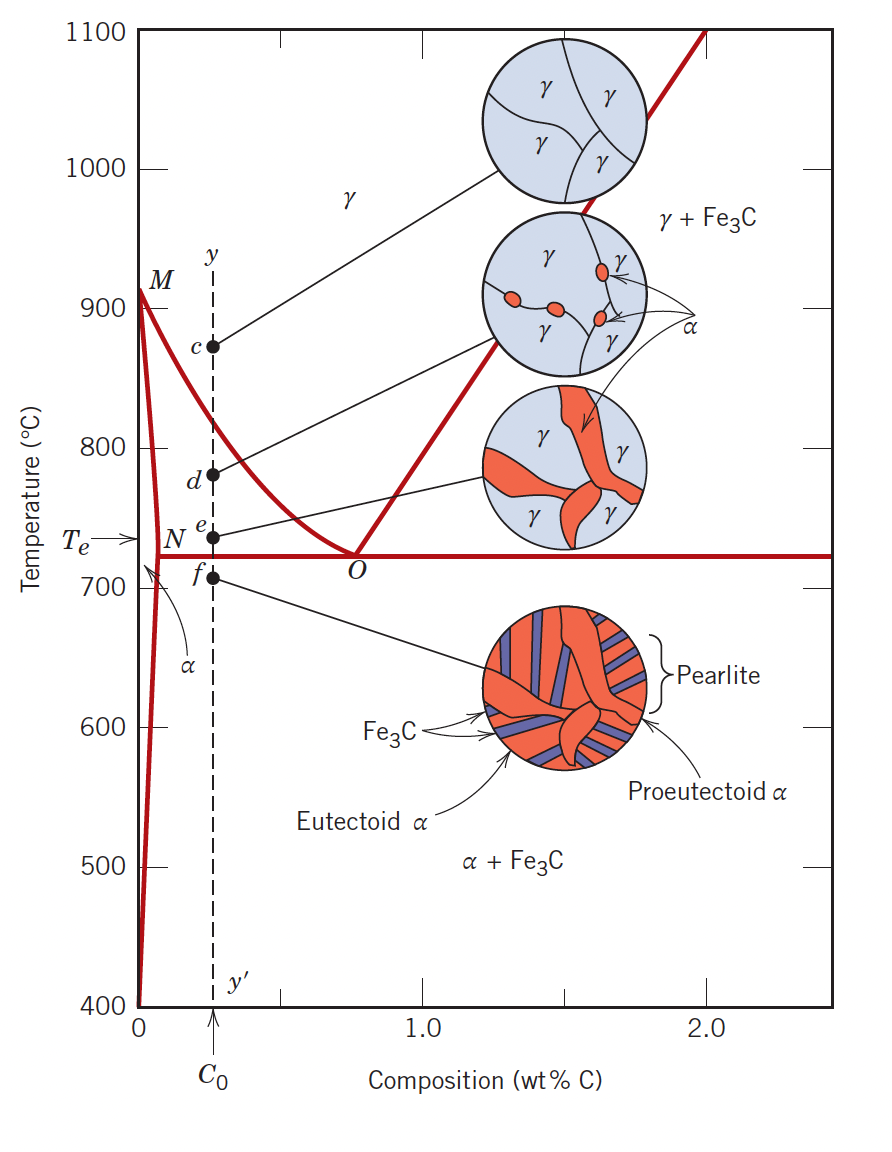
\includegraphics[width=0.35\linewidth]{./figures/f16_12.png}
  \caption{iron-iron carbon at hypoeutectoid composition}
  \label{fig:f16_12}
\end{figure}

While cooling an alloys through the $\alpha + \gamma$ phase region, the composition of the ferrite phase changes with temperature along the $\alpha-\left(\alpha + \gamma \right)$ phase boundary, line $MN$, is becoming slightly richer in carbon. However the change in composition of the austenite is more dramatic, proceeding along the $\left( \alpha + \gamma \right)-\gamma$ boundary, line $MO$. Cooling from point $d$ to $e$, just above the eutectoid but still in the $\alpha + \gamma$ region, produces an increased fraction of the $\alpha$ phase and a microstructure similar to that also shown: the $\alpha$ particles will have grown larger.

As the temperature is lowered just below the eutectoid, to point $f$, all of the $\gamma$ phase that was present at temperature $T_e$ transforms into pearlite. There is virtually no change in the $\alpha$ phase that existed at point $e$ in crossing the eutectoid temperature. The ferrite present in the pearlite is called \textit{eutectic ferrite}, whereas the other, which formed above $T_e$ is termed \textit{proeutectoid ferrite}. 

Something analagous is true for \textit{hypereutectic alloys} -- i.e. composition to the right of the eutectoid). Here pearlite is however not formed -- instead cementite is formed. 
